\documentclass[Protokollheft.tex]{subfiles}
\begin{document}
\chapter{Magnetostatik 2, Quasistatik und Frequenzbereich}
%--------------- Start Vorbereitungsaufgaben ---------------

Über einer leitenden Platte mit der Leitfähigkeit $\kappa=5.8\cdot10^7\,\text{S/m}$ und der Permeabilität $\mu=1000\,\mu_0$ befindet sich eine quadratische Stromschleife. 
Das Material des umgebenden Rechengebiet der festen Größe $1\,\text{m}\times1\,\text{m}\times1\,\text{m}$ ist Vakuum. 
Darüber hinaus gilt im gesamten Rechengebiet für die Permittivität $\varepsilon = \varepsilon_0$. 
Für eine äquidistante Diskretisierung der Größe $6\times6\times5$ ist diese Problemstruktur in Abbildung~\ref{fig:strukt} dargestellt.
Trotz der gewählten Allokation auf dualen Flächen ist der Strom hier für eine bessere Übersicht auf primären Kanten eingezeichnet.
Es sei in diesem Zusammenhang nochmal auf die Dualität des Gitters hingewiesen, die jeder primären Kante jeweils eine duale Fläche mit dem gleichen kanonischen Index zuordnet. 
Diese Diskretisierung eignet sich für das Testen der Implementierung. Insbesondere für die Visualisierungen sollte jedoch ein feineres Gitter verwendet werden.
Es sollen sinnvolle Randbedingungen verwendet werden. 
    \begin{figure}[ht!]
        \centerline{%
        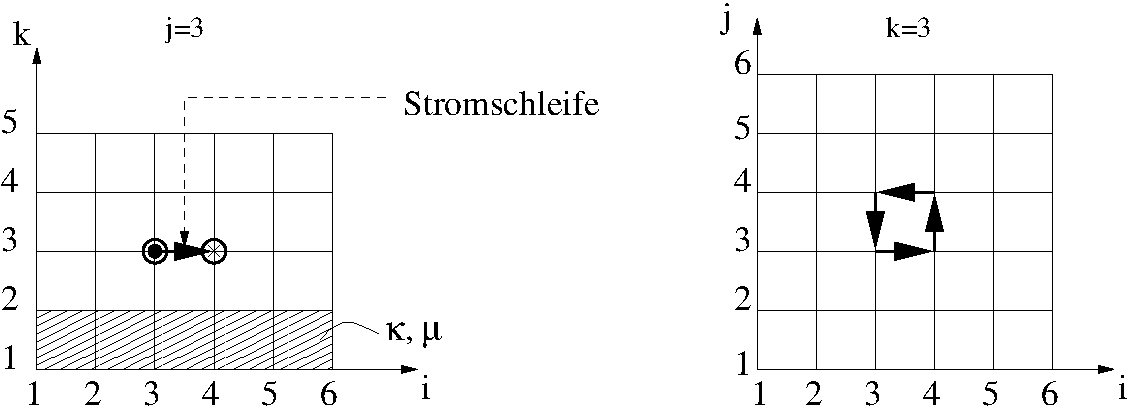
\includegraphics[scale=0.75]{v5_prakt3.pdf}
        }
        \caption{Problemstruktur. Gegeben ist ein äquidistantes, dreidimensionales Gitter. Die gestrichelt dargestellten Gitterzellen sollen mit leitfähigem Material gefüllt angenommen werden,
        d.\,h. $\kappa\neq0$ und $\mu\neq\mu_0$, der Rest der Gitterzellen ist Vakuum. Es gilt überall $\varepsilon=\varepsilon_0$. Im Versuch sollen allgemeine Diskretisierungen betrachtet werden. Bei feinerem Gitter gehen die Abmessungen von Schleife und Materialschicht entsprechend über mehrere Gitterzellen.}\label{fig:strukt}
    \end{figure}

\section{Vorbereitungsaufgaben}

% --> Aufgabe
\begin{framed}
	\noindent \textbf{1.} Bestimmen Sie für die Problemstruktur aus Abbildung~\ref{fig:strukt} die in FIT verwendeten
    gemittelten Leitfähigkeiten $\bar{\kappa}=(\bar{\kappa}_x\;\bar{\kappa}_y\;\bar{\kappa}_z)$ für die primalen Kanten, die von den primalen Punkten $P_{ik}$ für $(i,k)\in\{(3,1),(3,2),(3,3)\}$ ausgehen. Berechnen Sie zusätzlich die gemittelten inversen Permeabilitäten $\bar{\mu}^{-1}=(\bar{\mu}_x^{-1}\;\bar{\mu}_y^{-1}\;\bar{\mu}_z^{-1})$ für die dualen Kanten, die von den dualen Punkten $\widetilde{P}_{ik}$ mit $(i,k)\in\{(3,1),(3,2)\}$ ausgehen. Verwenden Sie zum Ermitteln dieser gemittelten Werte eine Taylorreihenentwicklung analog zu Versuch 3.\label{exer:averagedMaterials}
\end{framed}

Um die Werte zu bestimen, nutzt man die folgende 2 Formeln:
\begin{enumerate}
	\item Leitfähigkeit $\bar{\kappa}$
     bspl. Für x-Komponente
     \begin{eqnarray*} \bar{\kappa}_x(n)& = &\frac{1}{4\tilde{A}_x}(\kappa_x(n-M_y-M_z)A_x(n-M_y-M_z)\\
     &  &+\kappa_x(n-M_z)A_x(n-M_z)\\
     &    &+\kappa_x(n)A_x(n)\\
     &   &+\kappa_x(n-M_y)A_x(n-M_y))
    \end{eqnarray*}

 \item inversen Permäbilität $\bar{\mu}^{-1}$ bspl. für x-Komponente
$$\bar{\mu}_x^{-1}=\frac{\frac{\Delta x(n)}{2\mu(n)}+\frac{\Delta x(n-M_x)}{2\mu(n-M_x)}}{\Delta\tilde{x}(n)}$$ mit $$ \Delta\tilde{x}(n)=\frac{\Delta x(n-M_x)}{2}+\frac{\Delta x(n)}{2}$$
\end{enumerate}

So ergibt sich die Leitfähigkeiten zu:
\begin{enumerate}
	\item $(3,1) = (1\ 1\ 1) \cdot 5,8\cdot 10^7$S/m
	\item $(3,2) = (2,9\ 2,9\ 0)\cdot 10^7$S/m
	\item $(3,3) = (0\ 0\ 0)$
\end{enumerate}
Die inversen ermtivitäten auf den Dualen Kanten ergeben sich zu:
\begin{enumerate}
	\item $(3,1) = (1000\ 1000\ 500,5)\cdot \mu_0$
	\item $(3,2) = (\mu_0\ \mu_0\ \mu_0)$
\end{enumerate}

% --> Aufgabe
\begin{framed}
	\noindent \textbf{2.} Bestimmen Sie die Systemmatrix $\Amat_\text{F}$ des magnetoquasistatischen Problems im Frequenzbereich (Gleichung (5.14)).\label{exer:systemMatMQSF}
\end{framed}

Man nutzt die Gleichung (5.14):

$$ \curldfit\Mmui\curlfit\afit + j \omega\Mkap\afit = \jfit_{\boldmath{s}} $$
\begin{eqnarray}
\left[ \curldfit\Mmui\curlfit + j \omega\Mkap \right]\afit = \jfit_{\boldmath{s}} \\
\Amat_\text{F}\afit=\jfit_{\boldmath{s}}
 \end{eqnarray}
% --> Aufgabe
\begin{framed}
	\noindent \textbf{3.} Bestimmen Sie die Systemmatrix $\Amat_\text{T}$ des impliziten
      \textsc{Euler}-Zeitschrittverfahrens, d.h.\ setzen Sie die Näherung~(5.22) in das DAE-System~(5.7) ein und stellen Sie anschließend nach $\afit_{n+1}$ um.\label{exer:systemMatMQST}
\end{framed}
Man nutzt die Gleichungen (5.7)
$$ \curldfit\Mmui\curlfit\afit +           \Mkap      \frac{\partial }{\partial t}\afit = \jfit_{\boldmath{s}} $$
und (5.22)
$$ \frac{\partial }{\partial t}\afit(t_{i+1})=\frac{1}{\Delta t}\left(\afit_{i+1} - \afit_i\right).$$
Man setzt  Gleichung 5.22 in 5.7 ein
$$ \curldfit\Mmui\curlfit\afit_{i+1}+\frac{1}{\Delta t}\Mkap\left(\afit_{i+1} - \afit_i\right)= \jfit_{\boldmath{s}}. $$

Man stellt die Gleichung nach $\afit_{i+1}$ um:
$$ \left(\curldfit\Mmui\curlfit+\frac{1}{\Delta t}\Mkap\right)\afit_{i+1}= \jfit_{\boldmath{s}}+\frac{1}{\Delta t}\Mkap\afit_i. $$
Es ist deutlich zu sehen, dass $\Amat_\text{T} =\curldfit\Mmui\curlfit+\frac{1}{\Delta t}\Mkap $ ist.



% --> Aufgabe
\begin{framed}
	\noindent \textbf{4.}\label{3}
      Bei dem Vergleich einer Lösung im Zeitbereich mit der äquivalenten Lösung im Frequenzbereich stößt man auf das Problem, dass die Lösung im 
      Frequenzbereich einem komplexen Feldphasor entspricht, während die Lösung im Zeitbereich rein reellwertig ist. Man könnte nun den Realteil 
      des Feldphasors mit der Zeitbereichslösung vergleichen, kennt hier aber nicht die Phase des Phasors. Daher soll hier der Ansatz verfolgt werden, 
      aus dem Zeitsignal einen komplexen Phasor zu gewinnen und diesen mit dem Phasor aus der Frequenzbereichslösung zu vergleichen.
      
Stellen Sie nun geeignete Bedingungen für den unbekannten Realteil und Imaginärteil des komplexen Phasors auf, um diese zu bestimmen. Formen Sie daraufhin diese Beziehungen so um, dass Sie diejenigen Zeitpunkte erhalten, an denen Sie den Realteil und den Imaginärteil des Phasors direkt am eingeschwungenen Zeitsignal ablesen können.\label{exer:calcTimes4RealImag}
\end{framed}
\noindent
Betrachtet man die Zeitbereichslösung in Abhängigkeit eines Phasors so ergibt sich 
\begin{equation}
a(x,t)=\Re\{\underline{a}(x)\ e^{j\omega t}\}.
\label{eq:time_dom}
\end{equation}
Im Frequenzbereich kann man nun auch eine Gleichung aufstellen, indem man die Lösung in Real- und Imaginärteil aufteilt.
\begin{equation}
\underline{a}(x)=\underline{a}_{\Re}(x) +j\underline{a}_{\Im}(x)=|\underline{a}(x)|\ \text{cos}(\Phi)+j|\underline{a}(x)|\ \text{sin}(\Phi)
\label{eq:freq_dom}
\end{equation}
Nun soll derjenige Zeitpunkt $t^*$ ermittelt werden, an dem man den Real- und Imaginärteil des Phasors direkt am eingeschwungenen Zeitsignal ablesen kann.
Dazu verwendet man Gleichung \ref{eq:time_dom} und löst diese weiter auf. Man erhält:
\begin{equation}
a(x,t^*)=\Re\{\underline{a^*}(x)\ e^{j\omega t^*}\}=|\underline{a^*}(x)|\ \text{cos}(\omega t^*+\Phi).
\label{eq:time_dom_2}
\end{equation}
Um nun die Zeitpunkte $t^*$ erhalten muss man nun die Zeitbereichslösung aus Gleichung \ref{eq:time_dom_2} mit der Frequenzbereichslösung aus Gleichung \ref{eq:freq_dom} vergleichen. Das Ganze einmal für den Realteil und für den Imaginärteil.\\
\\
Realteil:
\begin{eqnarray*}
|\underline{a^*}(x)|\ \text{cos}(\omega t^*+\Phi)&=&|\underline{a^*}(x)|\ \text{cos}(\Phi)\\
\text{cos}(\omega t^*+\Phi)&=&\text{cos}(\Phi)\\
\omega t^*&=&2n\pi\\
t^*&=&\frac{n}{f}\\
t^*&=&nT
\end{eqnarray*}
\\
Imaginärteil:
\begin{eqnarray*}
|\underline{a}(x)|\ \text{sin}(\Phi)&=&|\underline{a}(x)|\ \text{cos}(\Phi-\frac{\pi}{2})\\
|\underline{a}(x)|\ \text{cos}(\Phi-\frac{\pi}{2})&=&|\underline{a^*}(x)|\ \text{cos}(\omega t^*+\Phi)\\
\text{cos}(\Phi-\frac{\pi}{2})&=&\text{cos}(\omega t^*+\Phi)\\
\omega t^*&=&2n\pi-\frac{\pi}{2}\\
t^*&=&nT-\frac{T}{4}
\end{eqnarray*}
\\
Es ergeben sich somit für den Realteil die Zeitpunkte $t^*_{\Re}=nT$ und für den Imaginärteil die Zeitpunkte $t^*_{\Im}=nT-\frac{\pi}{2}$, um die jeweiligen Phasoren am Zeitsignal ablesen zu können.

% --> Aufgabe
\begin{framed}
	\noindent \textbf{5.} Geben Sie für die Problemstruktur und unter der Voraussetzung, dass in der eingezeichneten Stromschleife ein Gleichstrom von $1\,\text{kA}$
      fließt, die Einträge des Stromdichtevektors $\jfit_\text{s}$ an. Bauen Sie den Stromdichtevektor $\jfit_\text{s}$ wie gewohnt mit dem kanonischen Indizierungsschema auf.\label{exer:calcCurrentExcitation}
\end{framed}
\noindent
Die Stellen, an denen der Stromdichtevektor $\jfit_\text{s}$ nicht Null Einträge besitzt, sind durch das kanonische Indizierungsschema gegeben. Somit kann man $\jfit_\text{s}$ direkt aufstellen.
\begin{eqnarray*}
	\jfit_\text{s}(87)&=&1000\ \text{A}\\
	\jfit_\text{s}(93)&=&-1000\ \text{A}\\
	\jfit_\text{s}(267)&=&-1000\ \text{A}\\
	\jfit_\text{s}(268)&=&1000\ \text{A}\\
\end{eqnarray*}

%Da nur in dem Leiterring ein Strom fließt, treten nur in den Edges Ströme und somit auch Stromdichten auf. So besteht der Stromdichtendvektor $\jfit$ aus Nullen, bis auf die Stellen 84 und 93 wo der Strom von $1000 \  \text A$ in Richtung der der Kanten Fließt und somit die Einträge gleich $1000$ sind. In den Indizes 267 und 268 hingegen fließt der Strom entgegen der Kantenrichtung und die Einträge sind somit $-1000$. 
% --> Aufgabe
\begin{framed}
	\noindent \textbf{6.}\label{loop}
      Zur Erstellung des elektrischen Feldes und der Wirbelstromdichte
      im impliziten Zeitbereichsverfahren muss nach Gl.~(5.9) die
      Zeitableitung des Vektorpotentials ausgewertet werden.
      Ein Ausdruck höherer Ordnung ensteht, indem für die
      Zeitableitung am \emph{halben} Zeitpunkt $t_{n+1/2}=(t_n+t_{n+1})/2$
      die beiden Näherungen
      \begin{align}\label{eq:approx1}
        \dot{\afit}_{n+1/2} &\approx \frac{\dot{\afit}_{n+1}+\dot{\afit}_n}{2} = \frac{-\efit_{n+1} - \efit_{n}}{2}, &\qquad\mbox{(arithmetisches Mittel)}\\
        \label{eq:approx2} \dot{\afit}_{n+1/2} &\approx \frac{\afit_{n+1} - \afit_{n}}{\Delta t} &\qquad\mbox{(zentraler Differenzenquotient)}
      \end{align}
      angesetzt werden.
    
      Leiten Sie durch Gleichsetzen beider Näherungen \eqref{eq:approx1} und \eqref{eq:approx2} und Auflösen nach
      $\efit_{n+1}$ eine Formel her, die die elektrische Gitterspannung
      in Abhängigkeit von ihrem jeweils letzten Wert und zwei
      Potentialwerten beschreibt.\label{exer:formulaEfit4pots}
\end{framed}
\noindent
Aus den Gleichungen \ref{eq:approx1} und \ref{eq:approx2} ergibt sich durch gleichsetzen
\begin{equation}
	\frac{-\efit_{n+1} - \efit_{n}}{2} \approx \frac{\afit_{n+1} - \afit_{n}}{\Delta t}
\end{equation}
Umstellen nach $\efit_{n+1}$ führt auf
\begin{equation}
	\efit_{n+1} = -2\frac{\afit_{n+1}-\afit_{n}}{\Delta t} - \efit_{n}
\end{equation}
% --> Aufgabe
\begin{framed}
	\noindent \textbf{7.} Weiterhin wird die Struktur aus Abbildung~\ref{fig:strukt} betrachtet. Überlegen Sie sich, wie
      $\Dkap$, d.\,h.\ die Matrix der Materialverteilung ohne Gitterabmessungen $\Delta s$ und $\Delta \widetilde{A}$, für eine allgemeine äquidistante Diskretisierung des Problems aussieht. Welcher Zusammenhang besteht zwischen dem elektrischen Gitterstrom und der elektrischen Gitterspannung? Welche Methode aus den letzten Versuchen
      müssen Sie daher nur leicht modifizieren, um die Materialmatrix $\Mkap$ zu erstellen?
      \label{exer:calcDkap}
\end{framed}
\noindent
Da für den Elektrische Gitterstrom der Zusammenhang $\jfit = \Mkap \efit$ gilt und dies sehr ähnlich ist mit $\dfit = \Meps \efit$ kann die Materialmatrix $\Mkap$ durch eine leicht modifizierte Funktion \lstinline{createMeps} erstellt werden. 
\\

%\emph{Fügen Sie hier Ihre Lösung ein}

\section{Aufgaben während der Praktikumssitzung}

    Alle Aufgaben dieses Versuchs benötigen die Modellierung des Problems, gegeben durch Gitter, Materialverteilung und Anregung.

% --> Aufgabe
\begin{framed}
	\noindent \textbf{1.} Modellieren Sie das Problem (siehe Abbildung~\ref{fig:strukt}), d.\,h.\ erstellen Sie das Rechengitter, die Anregung und die diskretisierten Materialverteilungen. Verwenden Sie hierzu das teilweise vorgegebene Skript \lstinline{versuch5.m}.\\
{\textbf{Hinweis:}} Beachten Sie, dass später die inverse Permeabilität benötigt wird.\label{exer:modelProblem}
\end{framed}

\emph{Fügen Sie hier Ihre Lösung ein}

%
Zuerst soll das magnetostatische Problem gelöst werden:
%

% --> Aufgabe
\begin{framed}
	\noindent \textbf{2.} Der Solver des magnetostatischen Problems mit Hilfe eines Vektorpotentials soll in der vorbereiteten Methode
          \begin{align}
                \lstinline{[hbow, bbow, relRes] = solveMSVec(msh, mui, jbow)} \label{pro:solveMsVec}
            \end{align}
            implementiert werden. Neben den bekannten Parametern \lstinline{msh} und \lstinline{jbow} ist \lstinline{mui} hier die diskrete, gemittelte, inverse Permeabilität.\label{exer:solveMSVec}
\end{framed}

\emph{Fügen Sie hier Ihre Lösung ein}

% --> Aufgabe
        \begin{framed}
	\noindent \textbf{3.} Erweitern Sie das Skript \lstinline{versuch5.m} und verwenden Sie Methode~\eqref{pro:solveMsVec} und \lstinline{plotEdgeVoltage}, um das magnetische Vektorpotential in der $x$-$y$-Ebene bei $k=3$ grafisch darzustellen. Visualisieren Sie außerdem die $z$-Komponente der magnetischen Flussdichte in der gleichen Schnittebene. Verwenden Sie hierfür den \lstinline{surf}-Befehl.\label{exer:visualizeMagVecPot}
\end{framed}
\begin{figure}
	\centering
	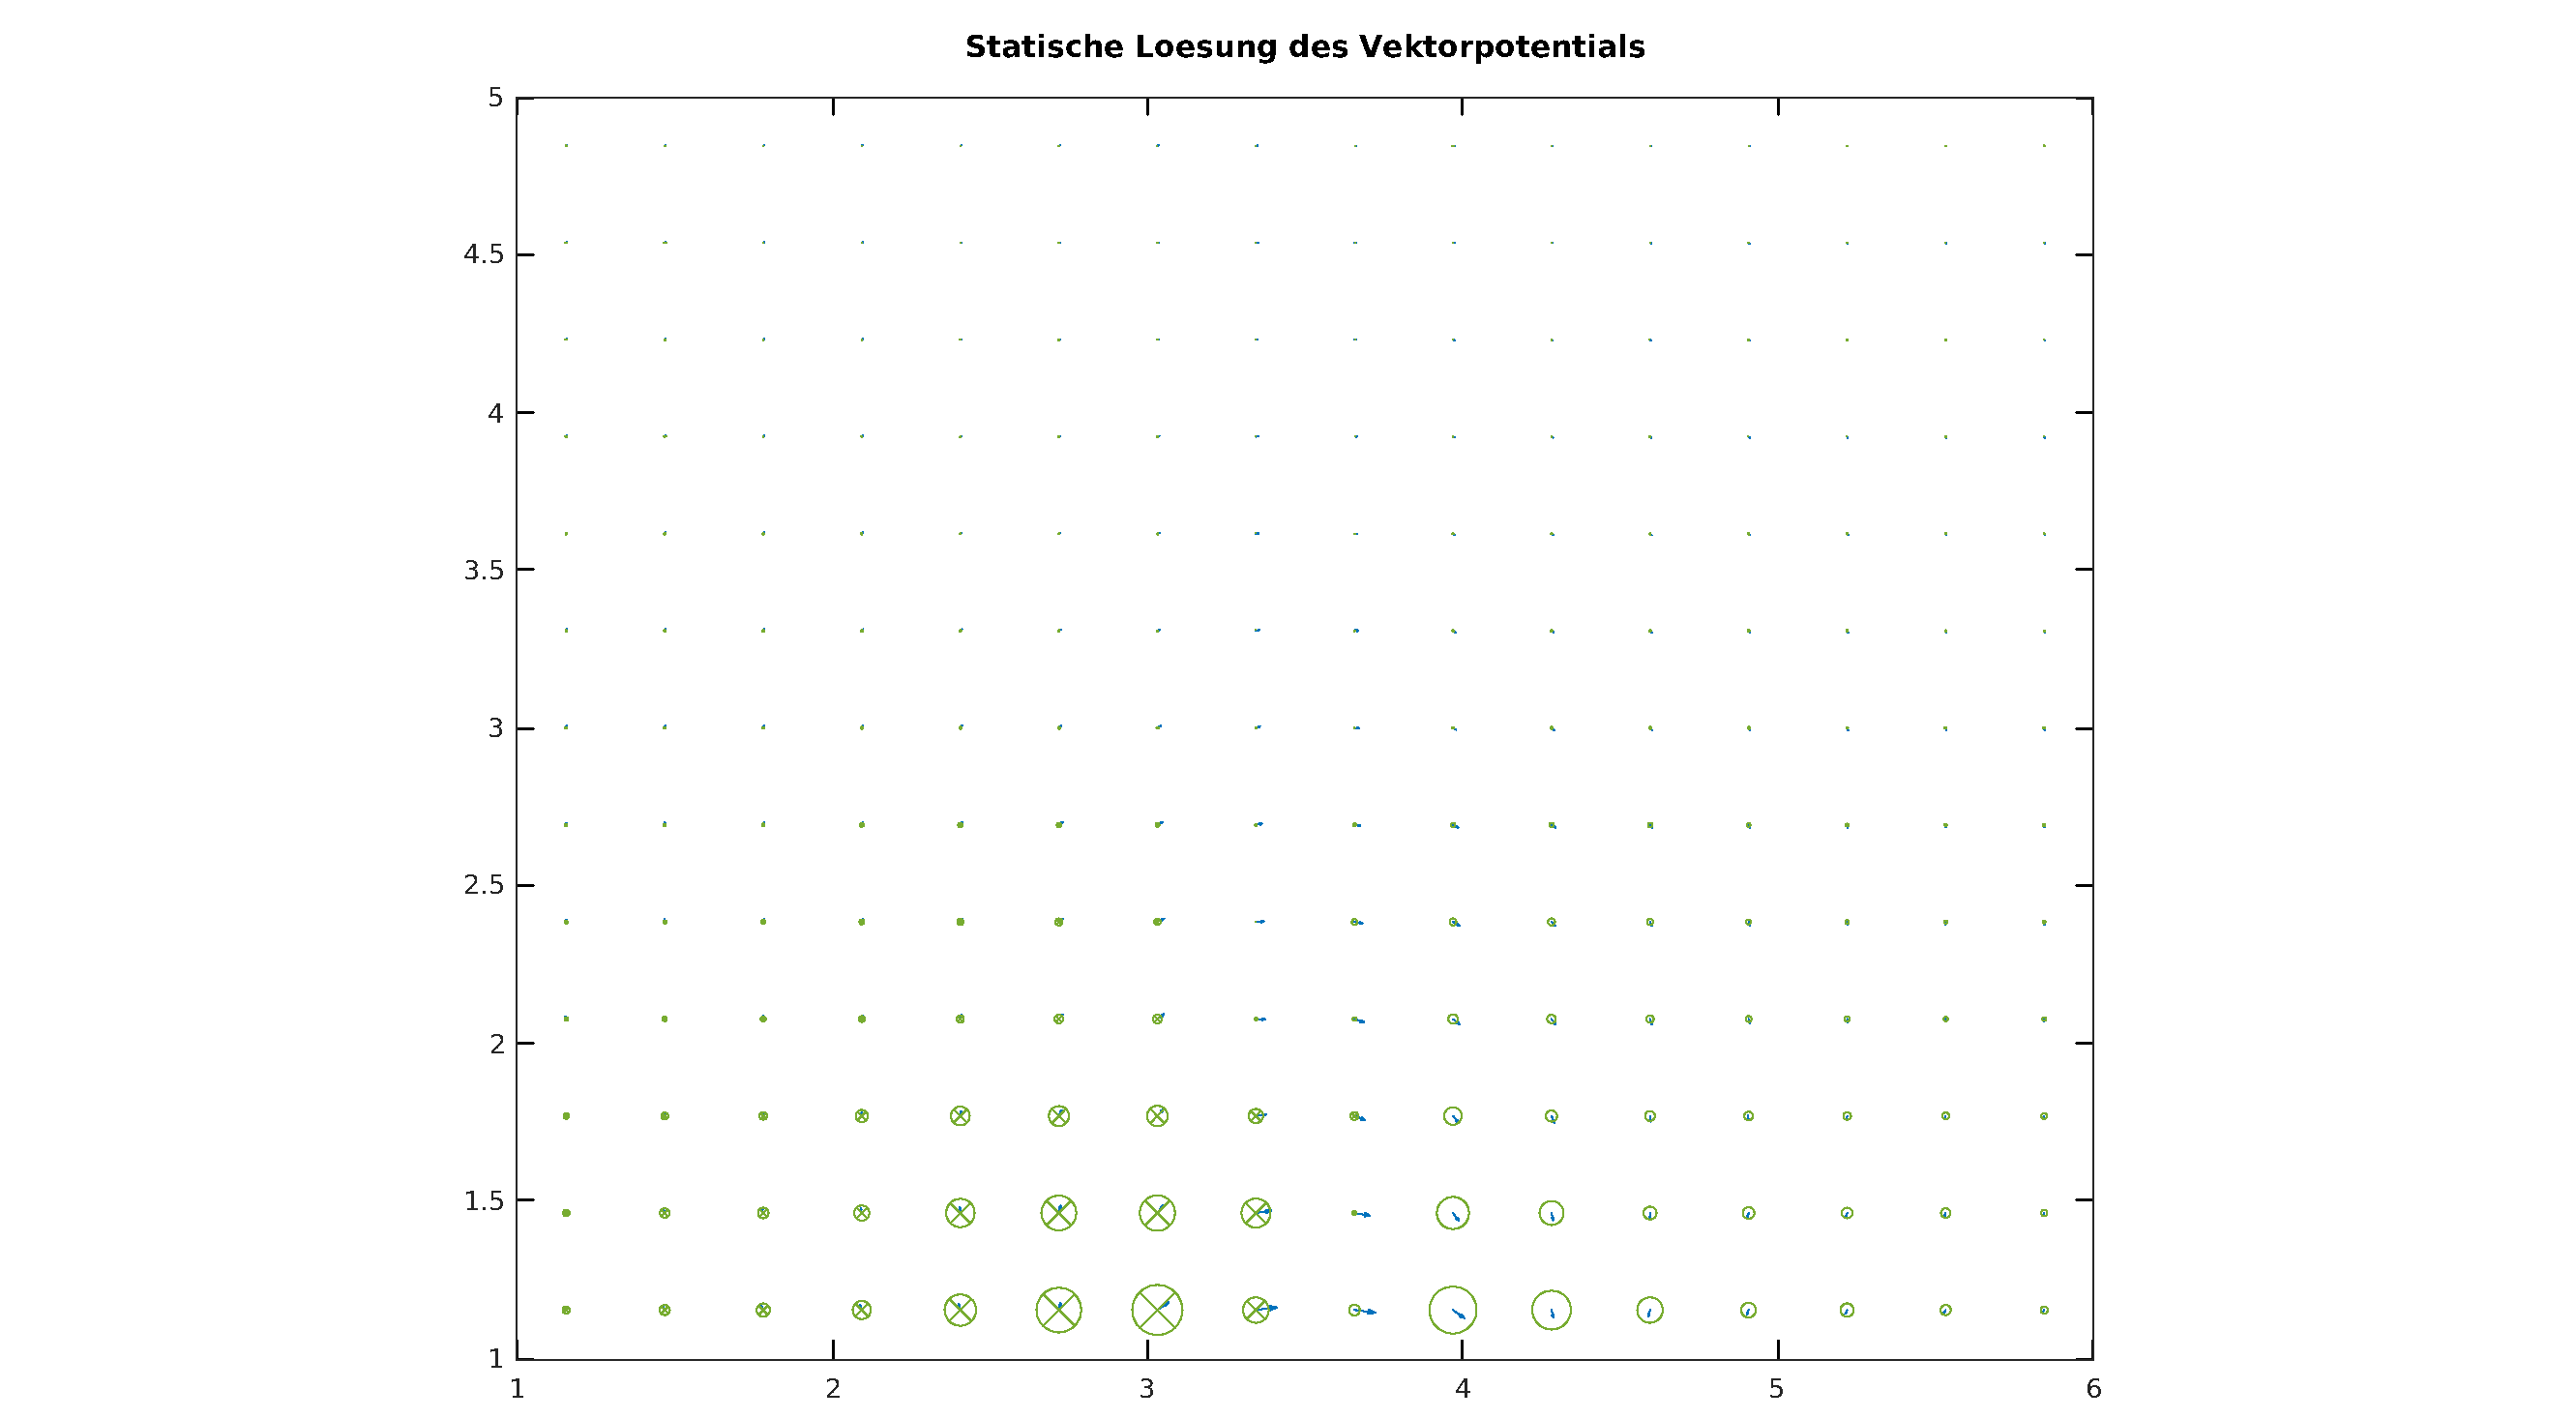
\includegraphics[width=0.7\linewidth]{StatischeLoesungdesVektorpotenzials.pdf}
	\caption{Statische Lösung des magnetischen Vektorpotenzials}
	\label{fig:statischeloesungdesvektorpotenzials}
\end{figure}

Das Vektorpotenzial des gegebenen Problems ist in Abb. \ref{fig:statischeloesungdesvektorpotenzials} dargestellt. Es ist eine Deutliche Überhöhung am unteren Rand des Rechengebietes zu erkennen. 
\\
%
Nun soll das Problem für eine harmonische Anregung bei der
Frequenz $f=50\,\text{Hz}$ gelöst werden:
%

% --> Aufgabe
\begin{framed}
	\noindent \textbf{4.} Implementieren Sie einen Solver für magnetoquasistatische Probleme im Frequenzbereich
          \begin{align}
                \lstinline{[hbow, bbow, jbow, relRes] = solveMQSF(msh, mui, kap, jebow, f)} \label{pro:solveMqs},
            \end{align}
            wobei \lstinline{kap} die diskrete, gemittelte Leitfähigkeit und \lstinline{f} die Frequenz der Anregung sind.\label{exer:solveMQSF}\\
            \ \\
            {\textbf{Hinweis:}} Beachten Sie dabei die korrekte Form der Systemmatrix $\Amat_\text{F}$ und der
            rechten Seite des Gleichungssystems. Das Gleichungssystem soll mit dem PCG-Verfahren
            gelöst werden (in \matlab\;gegeben als \lstinline{pcg}). Damit dieses konvergiert, müssen zunächst die Beiträge der Geisterkanten aus der Systemmatrix und der rechten Seite entfernt werden. Hierbei ist Ihnen die bereits gestellte Methode \lstinline{getGhostEdges} eine gute Hilfe. Außerdem muss ein geeigneter Vorkonditionierer (engl.\ preconditioner) gewählt werden. Besonders leicht zu implementieren ist z.B. der Jacobi Vorkonditionierer $\mathbf{M} = \text{diag}\,\Amat$.
\end{framed}


% --> Aufgabe
\begin{framed}
	\noindent \textbf{5.} Verwenden Sie Methode~\eqref{pro:solveMqs} in \lstinline{versuch5.m} und stellen Sie die Stromdichteverteilung in der Grenzfläche von Vakuum und leitender Platte als Vektorplot unter Verwendung von der gegebenen Methode \lstinline{plotEdgeVoltage.m} grafisch dar.\label{exer:currentDensityAtInterface}
\end{framed}


Des Weiteren soll dasselbe Problem im Zeitbereich mit dem impliziten
    \textsc{Euler}-Verfahren berechnet werden. Dazu muss ein
    Zeitintervall mit einer Schleife durchschritten werden.
    Das in jedem Schritt zu lösende Gleichungssystem haben Sie in der
    Vorbereitung hergeleitet.

% --> Aufgabe
\begin{framed}
	\noindent \textbf{6.} Es soll nun ein Solver im Zeitbereich implementiert werden:
      \begin{align}
            \lstinline{[hbow, bbow, jbow] = solveMQST(msh, mui, kap, jsbow, tend, nt)} \label{pro:solveT} \; ,
        \end{align}
        wobei \lstinline{t} der Simulationszeit und \lstinline{nt} der Zeitschrittanzahl entsprechen.\label{exer:solveMQST}
\end{framed}

\emph{Fügen Sie hier Ihre Lösung ein}

% --> Aufgabe
\begin{framed}
	\noindent \textbf{7.} Verwenden Sie Methode~\eqref{pro:solveT} und stellen Sie die Stromdichteverteilung im Punkt (3,2,2) in Abhängigkeit von der Zeit grafisch dar. Implementieren Sie diese Auswertung in \lstinline{versuch5.m}. Was erwarten Sie für grobe Diskretisierungen in der Zeit beim impliziten \textsc{Euler}-Verfahren als Vorteil gegenüber dem explizitem \textsc{Euler}-Verfahren?\label{exer:currDensityTimeDependent}
\end{framed}

\emph{Fügen Sie hier Ihre Lösung ein}

% --> Aufgabe
\begin{framed}
	\noindent \textbf{8.} Vergleichen Sie die Ergebnisse des Zeitbereichs-Solvers mit dem Ergebnis der Frequenzbereichslösung. Für diesen Vergleich muss die Frequenzbereichslösung zunächst in den Zeitbereich transformiert werden. Verwenden Sie anschließend für diesen Vergleich die Fehlernorm
      \begin{equation}
          \text{error} = \frac{\max||\bbow{\mathbf{j}}_\text{mqs,t}(t_i)-\bbow{\mathbf{j}}_\text{mqs,f,t}(t_i)||_2}{\max||\bbow{\mathbf{j}}_\text{mqs,f,t}(t_i)||_2}.
          \label{eq:errorNorm}
      \end{equation}
Die Zeitbereichslösung wird hier mit $\bbow{\mathbf{j}}_\text{mqs,t}$ und die in den Zeitbereich transformierte Frequenzbereichslösung mit $\bbow{\mathbf{j}}_\text{mqs,f,t}$ bezeichnet. Implementieren Sie diese Auswertung in \lstinline{versuch5.m}.\label{exer:compareFreqVStimeInTime}
\end{framed}


% --> Aufgabe
\begin{framed}
	\noindent \textbf{9.} Führen Sie nun denselben Vergleich noch einmal im Frequenzbereich durch. Hierfür müssen Sie den entsprechenden Phasor für die Zeitbereichslösung aufstellen und daraufhin den Real- und Imaginärteil mit der Frequenzbereichslösung vergleichen. Als Fehlernorm soll hier für Real- und Imaginärteil jeweils die Formel
    \begin{equation}
        \text{error} = \frac{||\bbow{\mathbf{j}}_\text{mqs,t,f}-\bbow{\mathbf{j}}_\text{mqs,f}||_2}{||\bbow{\mathbf{j}}_\text{mqs,f}||_2}
    \end{equation}
    verwendet werden. Die Frequenzbereichslösung wird hier mit $\bbow{\mathbf{j}}_\text{mqs,f}$ und die in den Frequenzbereich transformierte Zeitbereichslösung mit $\bbow{\mathbf{j}}_\text{mqs,f,t}$ bezeichnet. Implementieren Sie diese Auswertung in \lstinline{versuch5.m}.\label{exer:compareFreqVStimeInFreq}
\end{framed}


% --> Aufgabe
  \begin{framed}
	\noindent \textbf{10.} Stellen Sie die relativen Abweichungen nach~\eqref{eq:errorNorm} für mehrere Zeitintegrationen mit
      variierender Schrittweite in einem Skript \lstinline{plotConvSolveMQST} grafisch dar und beobachten Sie den entstehenden zeitlichen Diskretisierungsfehler. Bestimmen Sie die Ordnung des Zeitintegrationsverfahrens.\label{exer:relDiffMQSFvsMQST}
\end{framed}





\section{Fazit}
\emph{Fügen Sie hier Ihre Lösung ein}

\end{document}
